%--------------------------------------------------------------------
% NE 155 (intro to numerical simulation of radiation transport)
% Spring 2014

% formatting
\documentclass[12pt]{article}
\usepackage[top=1in, bottom=1in, left=1in, right=1in]{geometry}

\usepackage{setspace}
\onehalfspacing

\setlength{\parindent}{0mm} \setlength{\parskip}{1em}


% packages
\usepackage{amssymb}
%% The amsthm package provides extended theorem environments
\usepackage{amsthm}
\usepackage{epsfig}
\usepackage{times}
\renewcommand{\ttdefault}{cmtt}
\usepackage{amsmath}
\usepackage{graphicx} % for graphics files

% Draw figures yourself
\usepackage{tikz} 

% The float package HAS to load before hyperref
\usepackage{float} % for psuedocode formatting
\usepackage{xspace}

% from Denovo methods manual
\usepackage{mathrsfs}
\usepackage[mathcal]{euscript}
\usepackage{color}
\usepackage{array}

\usepackage[pdftex]{hyperref}

\newcommand{\nth}{n\ensuremath{^{\text{th}}} }
\newcommand{\ve}[1]{\ensuremath{\mathbf{#1}}}
\newcommand{\macro}{\ensuremath{\Sigma}}
\newcommand{\vOmega}{\ensuremath{\hat{\Omega}}}

\newcommand{\cc}[1]{\ensuremath{\overline{#1}}}
\newcommand{\ccm}[1]{\ensuremath{\overline{\mathbf{#1}}}}


%--------------------------------------------------------------------
%--------------------------------------------------------------------
\begin{document}
\begin{center}
{\bf NE 155, Classes 11 \& 12, S14 \\
Approximation and Interpolation \\ February 14 and 19, 2014}
\end{center}

\setlength{\unitlength}{1in}
\begin{picture}(6,.1) 
\put(0,0) {\line(1,0){6.25}}         
\end{picture}

%--------------------------------------------------------------------
Sometimes rather than calculating values of a function, we need to approximate them instead. Why might we do this?
%
\begin{itemize}
\item It may be difficult or impossible to analytically evaluate the function
\item We may have only a table of values at certain points and need to
determine the values in between
\item It may be much faster to compute values of an approximation
function than of the original function, particularly if we have to
calculate the function values over and over again
\item A function may be defined implicitly
\end{itemize}


%--------------------------------------------------------------------
%--------------------------------------------------------------------
\section{Approximation}
The approximation function does \underline{not}
need to fit through all given function values


%--------------------------------------------------------------------
\subsection{Types}
Usually, an approximating function is a linear combination of
simpler functions:
%
\begin{itemize}
\item $f(x)$: function to be approximated
\item $g(x)$: approximating function = $\sum_i a_i Ci(x)$
\end{itemize}
%
Examples
%
\begin{itemize}
\item \textbf{Polynomial}: $g(x) = P(x) = \sum_i a_i x^i$

\item \textbf{Piecewise polynomial}: slap some polynomials together so their ends meet

\item \textbf{Fourier series}: $g(x) = \frac{1}{2} a_0 + \sum_i [a_i \sin(ix) + b_i \cos(ix)]$ %http://mathworld.wolfram.com/FourierSeries.html

\item Combination of \textbf{rational functions}: $g(x) = R_n(x)/R_m(x)$

\item \textbf{Exponential functions}: $g(x) = \sum_i a_i \exp(b_i x^i)$
\end{itemize}

%--------------------------------------------------------------------
\subsection{Taylor Polynomial}
If $f(x)$ is known but difficult to evaluate, we can replace it by the
Taylor polynomial around x = a
\begin{align}
f(x) &= f(a) + f'(a)(a-x) + f''(a)\frac{(x-a)^2}{2!} + \cdots + f^{(n-1)}(a)\frac{(x-a)^{n-1}}{(n-1)!} + R_n \\
%
  &= \sum_{k=0}^{n-1}\frac{(x-a)^k}{k!}f^{(k)}(a) + R_n \\
%
R_n &= f^{(n)}(x^*)\frac{(x-a)^{n}}{n!} \qquad \text{for some } x^* \in [a, x]
%http://mathworld.wolfram.com/TaylorSeries.html
\end{align}

\begin{figure}[h!]
\begin{center}
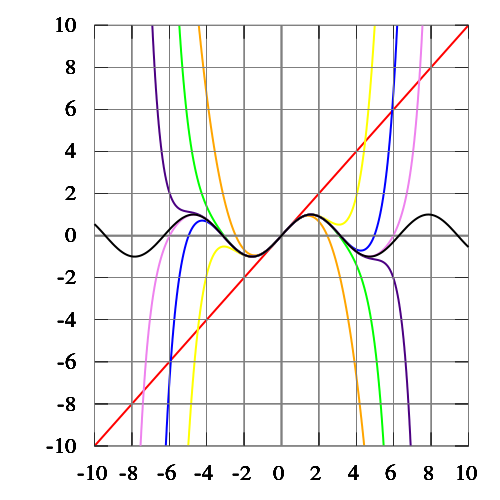
\includegraphics[height=3in,clip]{TaylorSinEg}
\caption{As the degree of the Taylor polynomial rises, it approaches the correct function. This image shows $\sin(x)$ and its Taylor approximations, polynomials of degree 1, 3, 5, 7, 9, 11 and 13.}
\end{center}
\end{figure}

%--------------------------------------------------------------------
\subsection{Lagrange Interpolating Polynomial}
If $x_0, x_1,\dots, x_n$ are $(n+1)$ distinct numbers and $f(x)$ is a function defined by these numbers, then there exists a unique polynomial $P(x)$ of degree at most $n$ with the property
%
\begin{align}
f(x_k) &= P(x_k)\:, \qquad \text{for }k= 0, 1, \dots, n \\
%
P(x) &= f(x_0)L_0(x) + \dots + f(x_n)L_n(x) = \sum_{k=0}^{n}f(x_k)L_k(x) \\
%
L_k(x) &= \prod_{i=0, i \neq k}^n \frac{(x-x_i)}{(x_k-x_i)}\\
%
L_k(x) &= \frac{(x-x_0)(x-x_1)\cdots(x-x_{k-1})(x-x_{k+1})\cdots(x-x_n)}{(x_k-x_0)(x_k-x_1)\cdots(x_k-x_{k-1})(x_k-x_{k+1})\cdots(x_k-x_n)}
\end{align}


\subsubsection{Error}
If $f$ is $n+1$ times continuously differentiable on a closed interval $I$

and $P_{n}(x)$ is a polynomial of degree at most $n$ that interpolates $f$ at $n + 1$ distinct points ${x_i}, (i=0,1,\dots,n)$ in that interval,

then for each $x$ in the interval there exists $\xi$  in that interval such that
%http://en.wikipedia.org/wiki/Polynomial_interpolation
\begin{align}
f(x) - P_n(x) &= \frac{f^{n+1}(\xi)}{(n+1)!}(x-x_0)(x-x_1)\cdots(x-x_n) \\
e &= \frac{f^{n+1}(\xi)}{(n+1)!}\prod_{i=0}^n (x-x_i)
\end{align}

The Lagrange polynomial of degree $n$ uses information at the
distinct numbers $x_0, x_1,\dots, x_n$ and, in place of $(x-x_0)^n$, its error formula uses a product of the $n+1$ terms.

%--------------------------------------------------------------------
%--------------------------------------------------------------------
\section{Interpolation}
The interpolation function does need to do
through all give values of the function.

%--------------------------------------------------------------------
%--------------------------------------------------------------------
%\bibliographystyle{plain}
%\bibliography{LinearSolns} 

\end{document}